\documentclass[12pt, titlepage]{article}
\usepackage{xcolor} % for different colour comments

%% Comments
\newif\ifcomments\commentstrue

\ifcomments
\newcommand{\authornote}[3]{\textcolor{#1}{[#3 ---#2]}}
\newcommand{\todo}[1]{\textcolor{red}{[TODO: #1]}}
\else
\newcommand{\authornote}[3]{}
\newcommand{\todo}[1]{}
\fi

\newcommand{\wss}[1]{\authornote{magenta}{SS}{#1}}
\newcommand{\ds}[1]{\authornote{blue}{DS}{#1}}

%% Graphics
\usepackage{float}
\usepackage{caption}
\usepackage{graphicx}
\graphicspath{ {Images/} }

\begin{document}

\title{Smart Waiter Detailed Design} 
\author{Meraj Patel \#1137491 \\ Pavneet Jauhal \#1149311\\ Shan Perera \#1150394}
\date{\today}
\maketitle

\tableofcontents 

\listoffigures

\listoftables


\section*{Template}
This document uses Volere Template for its organization.
\pagebreak

\section{Introduction}

\subsection{Purpose}
The purpose of Smart-Waiter aims to provide a solution that will allow users to order and pay through a mobile application at restaurants. 

\subsection{Description}
This opportunity arose from the lack of a universal application in the market that allows users to walk into a restaurant, scan a code to view the menu, and proceed to order and pay through the use of a singular application. Android users will be able to walk into any restaurant that offers our solution, and have the ability to use these services.

\subsection{Scope}
The scope of Smart-Waiter will be limited to providing the user with the following features: viewing the restaurant's menu, creating the user's order, placing the order and paying for their order. 
 
\section{Overview}

\subsection{Design Principals}
\subsubsection{Information Hiding}
Information hiding is the principle of segregation of design components that are likely to undergo changes as the lifecycle of the application progresses. This way, other key parts of the application will remain unhindered by any possible changes.

\section{Development Details}
\subsection{Language of Implementation}
The source code of the Android Smart-Waiter application will be written in Java and XML, as well as the API libraries used in development. 

\subsection{Supporting Frameworks/APIs}
CouchbaseLite (Database)
ZXing Embedded (QR Code Scanner)
Stripe (Credit Card)

\section{Implementation Components}
\subsection{Camera Function}
In this section we will detail the function that relates to the camera aspect of Smart-Waiter. There is one main function necessary for QR code scanning: onActivityResult. onActivityResult is called as soon as a QR code is captured by the camera. The function is passed three variables, a requestCode (int), a resultCode (int), an intent (Intent). Using these three variables, the function calls the ZXing function parseActivityResult using the three aforementioned variables as parameters. The parseActivityResult returns the contents of the QR code. 
 

function onActivityResult (requestCode, resultCode, intent)
	IntentResult contents = parseActivityFunction (requestCode, resultCode, intent)
	if(contents is not null)
		String QRContents = contents.getContents()
		Call populate menu functions using QRContents as a parameter
		
\subsection{Account Function}
In this section we will detail the key function that relates to account transactions and credit card charges. There is one key method related to credit card transactions: chargeParams, it involves using the Stripe class. As described in the System Architecture, given an instance of the Card class, and using Smart-Waiter's Stripe API key, a token is created and sent to the Stripe servers. The Stripe servers return a token that can be used to charge the user's credit card. The token is then used as a parameter of chargeParams, along with the information related to the credit card charge, like amount and the type of currency. 

Stripe = new Stripe (Smart-Waiter's Stripe API key)
createToken(card, tokenCallback())

token = request the Stripe token from Stripe server

try{
	chargeParams(amount, integer amount in cents)
	chargeParams(currency, string value of type of currency)
	chargeParams(source, token)
	chargeParams(description, string value of description regarding charges to card)

	charge = Charge.create(chargeParams)
}
catch (Exception e){
	Error handling
}
\subsection{Ordering Functions}
Below are function descriptions that are necessary for ordering in Smart-Waiter. As explained in System Architecture, there are three primary classes used to hold all vital information regarding menu information. These are: MenuCategories, MenuItems and User. These three classes are used to provide a user with a full menu of a particular restaurant and allow them to place an order.

\subsubsection{Parsing Function}
A parsing function was created to parse through received JSON response to save information in appropriate classes. Stated below is sudo code for this JSON parser. This function will parse through a JSON request. View if the key equals "categoryname". If so, save the value within MenuCategories class under . Also, if the key equals "categorypic" save the value within MenuCategories  class under pi

	function parse throws exception corrupt		
		define categoryArrayList 
		Save JSON response as list of hash map array
        for (each element in hash map list) {
            while (each  array element with list) {
                if(key equals categoryname){
                    Create MenuCategories object, save category name
                }
                if(key equals "categorypic"){
                    use MenuCategories object, save category name
                }
            }
            add created MenuCategories object to categoryArrayList
        }


\subsubsection{}


\section{User Interface Design}

\subsection{User Interface Design Overview}

\subsubsection{Menu Categories}
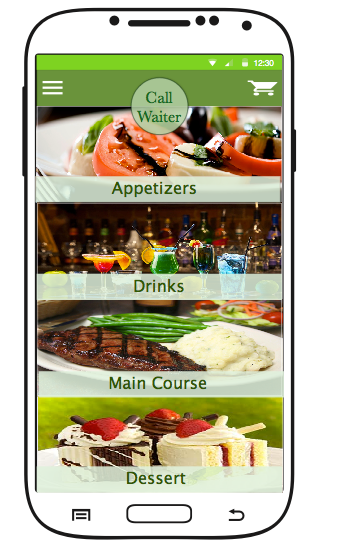
\includegraphics[width=80mm,scale=0.5]{MenuCategories.png}

\subsubsection{Menu Items}
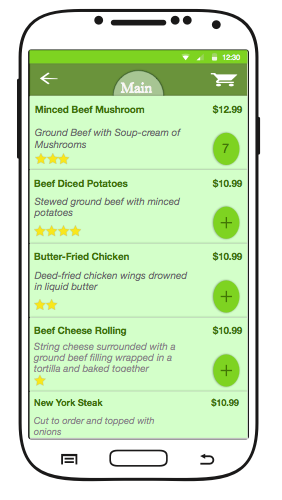
\includegraphics[width=80mm,scale=0.5]{CategoryItems.png}

\subsubsection{Confirm Order}
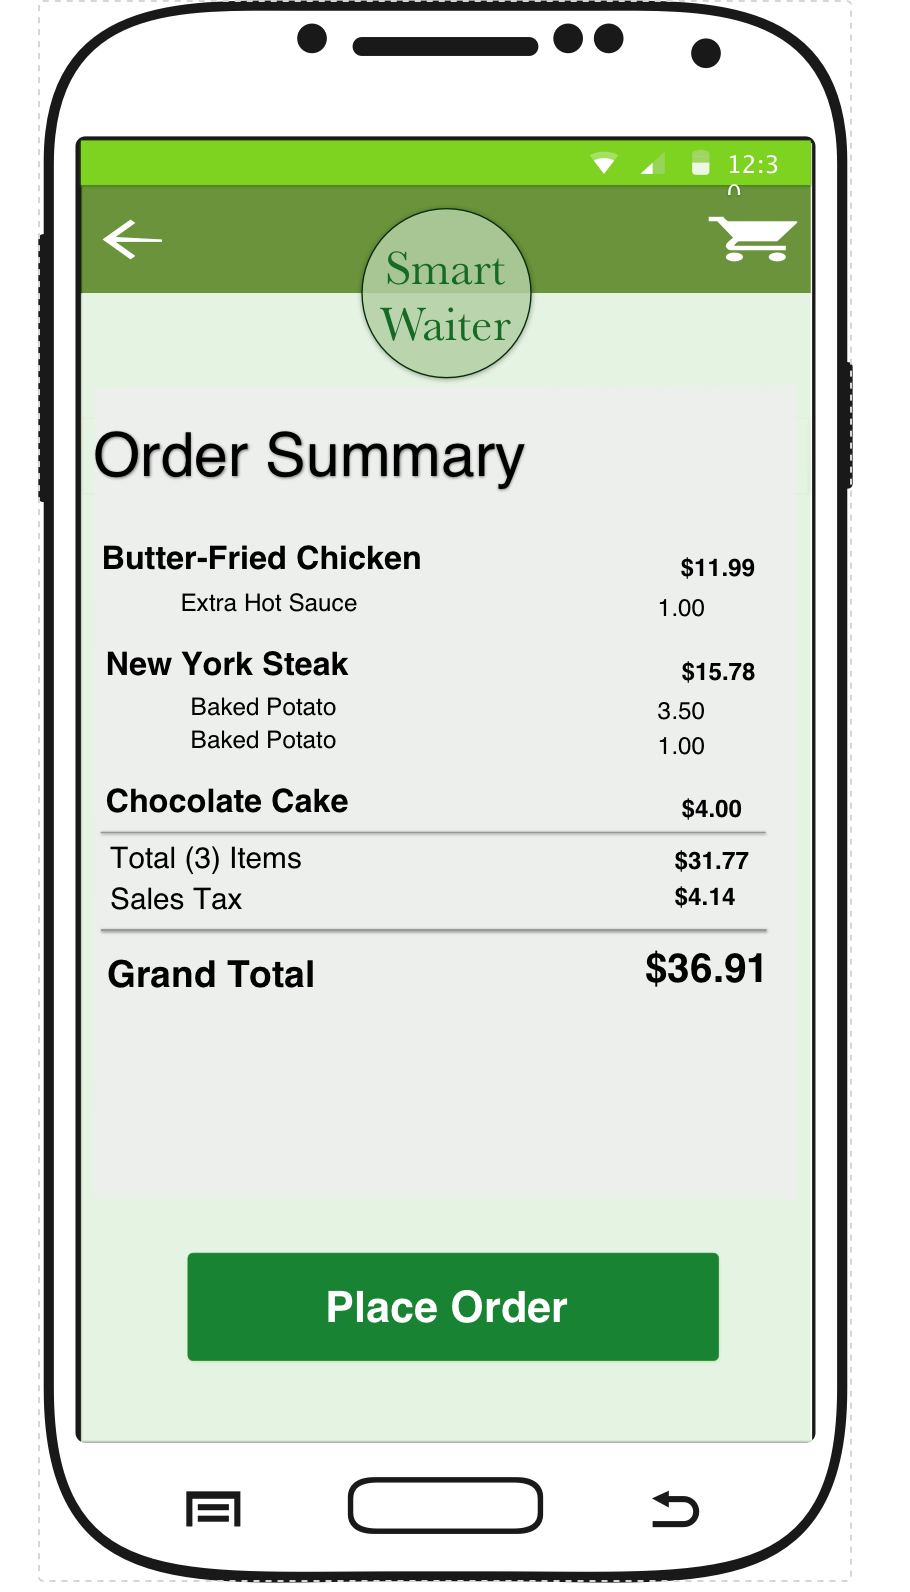
\includegraphics[width=80mm,scale=0.5]{OrderSummary.png}

\subsection{User Interface Navigation Flow}

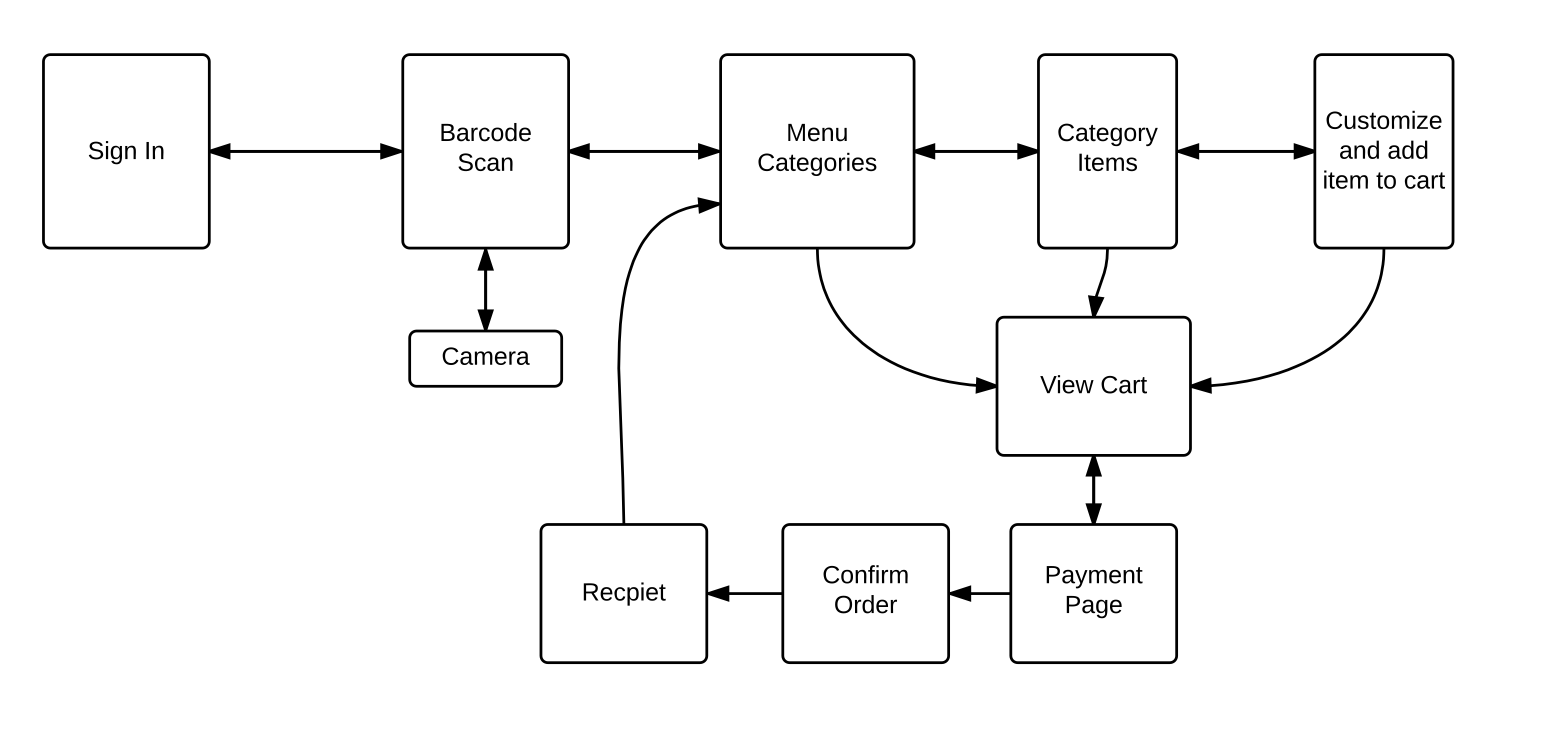
\includegraphics[width=180mm,scale=0.5]{UIProcess.png}

\subsection{Use Cases}

\subsubsection{Sign In Page}
\begin{center}
    \begin{tabular}{ | l | p{8cm} |}
    \hline
    User Input & System Response \\ \hline
    Enters correct user name and password & Application transitions to Barcode Scan page \\ \hline
    Enters incorrect user name and password & Toaster displayed reading "incorrect login, please try again" \\ \hline
    Enters incorrect user name & Toaster displayed reading "incorrect login, please try again" \\ \hline
    Enters incorrect password & Toaster displayed reading "incorrect login, please try again" \\ \hline
    Clicks "Skip Sign in" & Application  transitions to Barcode Scan page\\ \hline
    Clicks Back Button on phone & Application Quits \\
    \hline
    \end{tabular}
\end{center}


\subsubsection{Barcode Scan Page}
\begin{center}
    \begin{tabular}{ | l | p{10cm} |}
    \hline
    User Input & System Response \\ \hline
    Clicks Scan Barcode & Application transitions to camera so user can scan code. If successful, application will transition to menu page. Otherwise will return to scanning page and display a toaster reading, "please try again" \\ \hline
    Clicks back button on phone & Application transitions to Sign in Page \\
    \hline
    \end{tabular}
\end{center}

\subsubsection{Menu Categories Page}
\begin{center}
    \begin{tabular}{ | l | p{10cm} |}
    \hline
    User Input & System Response \\ \hline
    Clicks category & Application transitions Category Items \\ \hline
    Clicks back button on phone & Application transitions to Barcode Scan \\
    \hline
    \end{tabular}
\end{center}

\subsubsection{Category Items Page}
\begin{center}
    \begin{tabular}{ | l | p{10cm} |}
    \hline
    User Input & System Response \\ \hline
    Clicks Item & Application transitions to Customize Item \\ \hline
    Clicks back button on phone & Application transitions to Menu Categories \\
    \hline
    \end{tabular}
\end{center}


\subsubsection{Customize Item Page}
\begin{center}
    \begin{tabular}{ | l | p{8cm} |}
    \hline
    User Input & System Response \\ \hline
    Ticks check boxes & None \\ \hline
    Enters special instructions in input field & None \\ \hline
    Clicks "Add to Cart" & Transitions to cart page and populate list with item \\ \hline
    Clicks back button on phone & Application transitions to Menu items \\
    \hline
    \end{tabular}
\end{center}

\subsubsection{Cart Page}
\begin{center}
    \begin{tabular}{ | l | p{10cm} |}
    \hline
    User Input & System Response \\ \hline
 	Clicks "Delete" &  Deletes item from list\\ \hline
    Clicks "Submit Order" &  Transitions to payment page\\ \hline
    Clicks back button on phone & Application transitions to previous page \\
    \hline
    \end{tabular}
\end{center}

\subsubsection{Payment Page}

\begin{center}
    \begin{tabular}{ | l | p{7cm} |}
    \hline
    User Input & System Response \\ \hline
 	Input valid credit card and clicks "Process" & Transitions into Confirm Order page \\ \hline
    Input invalid credit card and clicks "Process" &  Toaster displayed reading "invalid credit card"\\ \hline
    Clicks back button on phone & Application transitions to previous Cart Page \\
    \hline
    \end{tabular}
\end{center}



\end{document}
